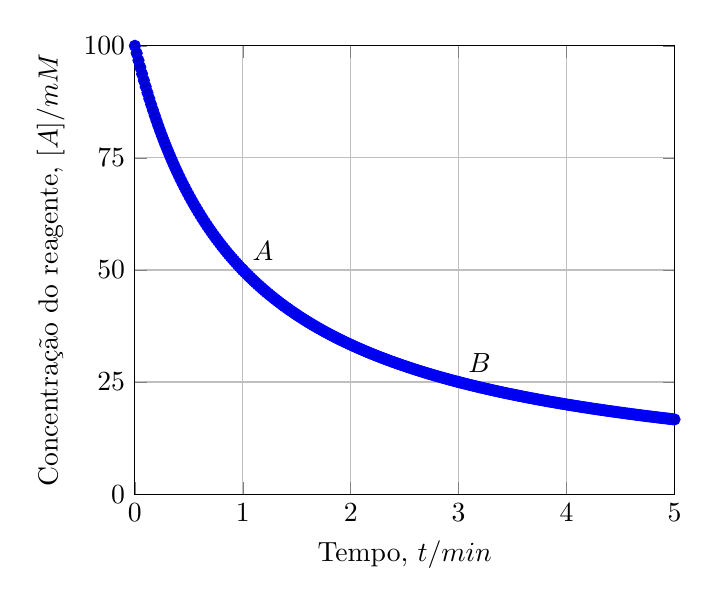
\begin{tikzpicture}
    \begin{axis}
        [
            xlabel = {Tempo, $t/\unit{min}$},
            ylabel = {Concentração do reagente, $[\ce{A}]/\unit{mM}$},
            ymin = 0, ymax = 100,
            xmin = 0, xmax = 5,
            domain = 0:5,
            grid = major,
            samples = 300,
            ytick = {0, 25, 50, 75, 100},
        ]

    \addplot+ [ blue ]
        {
            1/(1/100 + x/100)
        };

    \addplot [ mark=*, color=blue, only marks ] coordinates
        { 
            (1, 50) 
            (3, 25) 
        };
    
    \node [anchor = south west] at (axis cs:1,50) 
        {$A$};

    \node [anchor = south west] at (axis cs:3,25) 
        {$B$};

    \end{axis}
\end{tikzpicture}